\section{Aktivitetsmålere til børn} \label{tracker_intro}
%%Den gamle intro
%\textit{Dette afsnit omhandler, en beskrivelse af funktionaliteten for en række udvalgte aktivitetsmålere. Disse aktivitetsmålere bliver vurderet og analyseret på baggrund af opstillede succeskrav. Afslutningsvis præsenteres den samlede vurdering af aktivitetsmålerne, og hvordan disse opfylder opstillede kriterier.}
\textit{Dette afsnit omhandler optimale egenskaber for en aktivitetsmåler samt funktionaliteten af nuværende aktivitetsmålere til børn. Hertil vil en række udvalgte aktivitetsmålere blive vurderet og analyseret på baggrund af opstillede succeskriterier. Afslutningsvis præsenteres den samlede vurdering af aktivitetsmålerne, og i hvilken grad disse opfylder de opstillede kriterier.}
%%Gammel indledning 
%
%Sundhedsstyrelsen anbefaler børn at motionere 2,5 ugentligt, hvis dette ikke opfyldes karakteriseres barnet som inaktivt. Manglende motion kan være som resultatet af den teknologiske udvikling, som medfører en mere stillesiddende livsstil. \citep{ObesityActionCoalition} Den teknologiske udvikling som medvirker til inaktivitet og stillesiddende livsstil, er forsøgt udnyttet som modarbejdende faktor. Flere producenter har benyttet teknologi som et led i at motivere børn til et mere aktivt liv \citep{Fuhu2015,PowerAbout2015}. Fælles for disse producenter er, at de motiverer børn til at fysisk aktivitet gennem spil og leg. Producenterne benytter aktivitetsmålere til at registrere aktivitet. Sideløbende belønnes børnene med et antal point, afhængigt af aktivitetsniveauet. Børnene har i mange tilfælde mulighed for at spille alene, men også i hold. Dette medfører en mulig implementering af motions motiverende teknologier i et skoleregi. \newline
%Potentialet af en teknologi som motiverer børn til en aktiv livsstil kan have flere fordele. Den primære fordel ved en aktiv livsstil er forebyggelsen af følgesygdomme. Dette har vist sig at være en fordelagtig økonomisk og sundhedsmæssig investering.
%% Ny indledning
\subsection{Succeskriterier for aktivitetsmålere} \label{succeskrav}
Den teknologiske udvikling kan være medvirkende til inaktivitet og en stillesiddende livsstil. Flere producenter har dog benyttet teknologi, i form af aktivitetsmålere, som et led i at motivere børn til et mere aktivt liv gennem spil og leg. Børnene har i mange tilfælde mulighed for at spille alene men også i sociale sammenhænge.  %, hvorfor det er muligt at implementere aktivitetsmotiverende teknologier i et skoleregi. 
\citep{Fuhu2015,PowerAbout2015} Denne sammenkobling af teknologi og fysisk aktivitet er blandt andet udnyttet af firmaet Playware, som har haft positive resultater hvad angår motivering til øget fysisk aktivitetsniveau \citep{Rishoej2010}. Yderligere giver autonom fysisk aktivitet med intrinsisk motivation det bedste udbytte for børn \citep{J.Sebire2013}. \newline
En teknologi, som motiverer børn til en aktiv livsstil, har potentielt flere samfundsøkonomiske og sundhedsmæssige fordele, idet en aktiv livsstil blandt andet er forebyggende for diverse af følgesygdomme, som beskrevet i \secref{subsec:inover}. \newline


Aktivitetsmålere til børn bør tage højde for en række essentielle kriterier, som blandt andet indebærer at alt barnets daglig aktivitet registreres. Dermed skal barnets samlede fysisk aktivitet i løbet af en dag, indeholdene fritidsaktiviteter såvel som skolerelaterede aktiviteter, kunne registreres og gemmes af systemet.  %Nævnt i \secref{subsec:fysio_aktivitet} anbefales det, at børn dagligt udfører 60 minutters aktivitet med moderart til høj intensitet. 
Et studie har endvidere undersøgt hvilke børneidrætter der er de 10 mest populære blandt børn i aldersgruppen 7-15 år. Det fremgår af dette studie, at syv ud af de 10 mest populære børneidrætter involverer gang eller løb \citep{Asserhoej2013}. Desuden fremgår det af flere  studier, at cykling er en af hyppigst benyttede transportmidler for børn i alderen 10-15 år \citep{DTU2014,COWI2015}. \newline
På baggrund af ovenstående betragtninger, skal en aktivitetsmåler kunne registrere gang, løb og cykling for dermed at kunne bestemme barnets samlede fysiske aktivitetsniveau i løbet af en dag. Ydermere skal aktivitetmåleren derfor automatisk kunne skelne mellem aktivitetsformerne; gang, løb og cykling. Denne automatiske genkendelse af hvilken aktivitet der udføres, skal udformes ved brug af flere forskellige sensorer. Herved kan aktivitetsmåleren opnå en stor brugervenlighed, idet barnet ikke selv skal indtaste hvilken type aktivitet der vil blive udført. \newline
Intensiteten af en given fysisk aktivitet kan desuden bestemmes af en persons puls, som det fremgår i afsnit~\secref{subsec:fysio_aktivitet}. Dermed skal en aktivitetsmåler ligeledes kunne bestemme barnets puls, og dermed kategorisere hvilken intensitet som den fysiske aktivitet er udført med.


%Idet aktivitetsmåleren skal anvendes igennem en skoledag, så skal aktivitetsmåleren også kunne registrere aktivitetsformer, der er tilgængelige i skolen. Sundhedsstyrelsen har opstillet en række aktivitetsformer, hvor det ønskede intensitetsniveau opnås. Aktivitetsformer, som er tilgængelige for børn igennem en skoledag, er eksempelvis lege, der indebærer løb, leg i skolegården, cykling, fodbold og basketbold. Fælles for disse aktivitetsformer er, at de kan registreres som gang, løb og cykling. \citep{Sundhedsstyrelsen2003}
%I takt med at den daglige aktivitet opfanges bør en aktivitetsmåler kunne registrere, og dermed også adskille, gang, løb og cykling, hvilket gøres gennem forskellige sensorer.
 
%For at en aktivitetsmåler kan registrere aktivitet, kræves det at aktivitetsmåleren indeholder sensorer. Med den rette algoritme kan sensorer automatisk skelne mellem de nævnte former for aktivitet. 
%Idet de fysiologiske effekter i forbindelse med aktivitet er forskellige alt efter intensitetsniveauet, skal aktivitetsmåleren ydermere kunne registrere intensiteten af aktiviteten og belønne brugeren gennem brugerfladen.  

Målgruppen for den tilsigtede aktivitetsmåler er, som beskrevet i afsnit~\secref{sec:maalgruppe}, børn i aldersgruppen 9-12 år. Endvidere har afsnit~\secref{motivation_boern} påvist, at børn i den valgte målgruppe motiveres mest optimalt til  gennem autonom fysisk aktivitet med intrinsisk motivation, såsom leg og spil. Aktivitetsmåleren skal derfor kunne benytte sig af en type motivation som henvender sig til målgruppens behov. \newline

Aktivitetsmåleren placering og påmontering på en person skal desuden være komfortabel. Aktivitetsmåleren må dermed ikke fratage eller hindre barnets psykisk såvel som fysiske udfoldelse, i forbindelse med benyttelsen af denne. 

%Da aktivitetsmåleren skal benyttes hovedsageligt af inaktive børn, skal den kunne motivere til fysisk aktivitet. Ifølge \secref{motivation_boern} tyder det på, at børn i den udvalgte målgruppe motiveres til aktivitet gennem leg og spil. Et essentielt kriterie vil derfor være at kunne motivere denne målgruppe uanset alder og køn. \newline
%En aktivitetsmåler skal ikke være til gene, da en eventuelt gene i forbindelse med placeringen muligvis vil medføre fravalg af benyttelse og derved fysisk aktivitet. Derfor er et yderligere kriterie, at aktivitetsmåleren ikke skal være til gene. Børnene med en aktivitetsmåler påsat skal være lige så frie som foruden.

Den optimale aktivitetsmåler skal dermed kunne: 
\begin{itemize}
\item Registrere gang.
\item Registrere løb.
\item Registrere cykling.
\item Registrere aktivitetens intensitet. %igennem puls
\item Motivere både fysisk inaktive og fysisk aktive børn. %socialt
\item Monteres og placeres på komfortabel vis.
\end{itemize}

\subsubsection{Afgrænsning af aktivitetsmålere}  %Hed før Baggrund for analyse og vurdering af aktivitetsmålere
Der er udvalgt fire aktivitetsmålere til videre analyse, som alle har tilnærmelsesvis samme formål; at motivere børn til et øget fysisk aktivitetsniveau. De udvalgte aktivitetsmålere henvender sig alle til børn i målgruppen 9-12 år, og har derfor på forskellig vis udformet en brugerflade som er motiverende for målgruppen. Ydermere er aktivitetsmålerne trådløse og tilbyder, gennem trådløs overførsel, en brugerflade i form af en hjemmeside eller app. \newline
De udvalgte aktivitetsmålere vil blive analyseret og vurderet på baggrund af ovenstående opstillede succeskriterier.

\subsection{UNICEF kid power band}
UNICEF Kid Power Band er en aktivitetsmåler, som appellerer til børn ved at hjælpe andre børn i ressourcefattige lande, hvoraf sloganet til aktivitetsmåleren udspringer; "Vær aktiv. Red liv". \newline
Aktivitetsmåleren, der er udformet som et armbånd, fremgår af~\figref{fig:unicef}. Aktivitetsmåleren benytter et pedometer og et accelerometer til at registrere barnets fysiske aktiviteter. \citep{PowerAbout2015,PowerManual2015}

\begin{figure}[H]
	\centering
	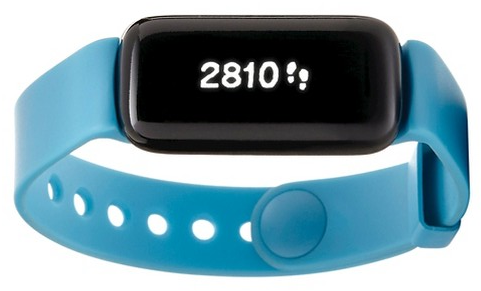
\includegraphics[scale=0.6]{figures/aProblemanalyse/unicef.png}
	\caption{På figuren ses UNICEF kid power band. \cite{Unicef2016}}
	\label{fig:unicef}
\end{figure}

Børnene kan optjene point ved at være fysisk aktive - desto mere fysisk aktive de er, desto flere point samler de sammen. Pointene omregnes til en sum penge, som sponsoreres af fans, firmaer og forældre. Pengene som børnene dermed gør sig fortjent til gennem fysisk aktivitet, vil blive sendt til de resourcefattige lande som aktivitetsmåleren støtter. \newline
Børnene har mulighed for at vælge mellem en række udvalgte lande, gennem såkaldte missioner. Disse missioner handler om, at lære børnene om samfundet i det pågældende land og dermed giver børnene indsigt i hvor betydningsfuld deres hjælp er. Børnene har gennemført en enkelt mission, når de har været fysisk aktive nok til at have optjent alle point for den pågældende mission. \newline
Alle resultater samles i en app, hvor børnene både har mulighed for at følge med i progressionen for dem selv og deres venner, samt for de missioner de deltager i. \citep{PowerAbout2015, PowerManuel2015}

%For at optjene point, skal børnene gennemføre forskellige missioner, som professionelle atleter står i spidsen for, hvorigennem børnene ikke blot er aktive men også lærer om forskellige kulturer.\fxnote{Et eksempel er en mission, som basketballspilleren Tyson Chandler står i spidsen for, hvor børnene lærer om hvordan børn i ressourcefattige lande, hjælper familien med at gro deres eget mad.} \citep{PowerMission2015} 
%Børnene kan selv følge med i, hvor langt de er i den pågældende mission på aktivitetsmåleren eller gennem en applikation (app). Når børnene har gennemført en mission, omregnes deres point til en sum penge, sponsoreret af fans, firmaer og forældre, som sendes til det pågældende ressourcefattige land, som missionen støtter. \newline
%Hver dag nulstilles aktivitetsmåleren, så børnene hver dag kan følge med i hvor aktive de har været den pågældende dag. Derudover gemmes der data 30 dage tilbage, så det er muligt at sammenligne med tidligere dage. 
%På aktivitetsmåleren er der en skærm, hvor det er muligt at følge med i klokken, antal skridt, KidPower points, fremskridt på missioner og navnet på brugeren. 
%Alle resultater samles i en applikation (app), hvor børnene både har mulighed for at følge med i progressionen for dem selv og deres venner, samt for de missioner de deltager i. \citep{PowerAbout2015}


\subsubsection{Vurdering af succeskriterier}
Aktivitetsmåleren giver mulighed for at tælle skridt, som både registreres under løb, gang og andre aktiviteter, dog skelnes der ikke mellem aktiviteterne. Da armene ikke bevæges ved cykling, er dette ikke muligt for aktivitetsmåleren at registrere. Derudover måles intensitet af det udførte arbejde ikke, idet der udelukkende måles hvor energisk armene bevæges under en givne øvelse, og ikke puls, iltoptagelse eller anstrengelse. Aktivitetsmåleren er designet som et armbånd, som nemt kan sættes på barnet, da den har en justerbar rem. \citep{PowerManual2015} \newline
Børnene udfører de fysiske aktiviteter sammen med andre børn, med henblik på at hjælpe børn i ressourcefattige lande. Aktivitetsmåleren motiverer børnene på intrinsisk vis, grundet de sociale aspekter som ligger til grund for aktivitetsmålerens brugerflade. \newline
Aktivitetsmåleren har desuden en indkøbspris på XXXXX kr.
%Børnene aktiveres socialt, da alle aktiviteter udføres med henblik på at de sammen med jævnaldrende, skal hjælpe børn i ressourcefattige lande. Derudover bliver børnene gennem appen opdateret på progression i de missioner de deltager i, samt venners progression, hvorved det ikke kun er den individuelle præstation der er i fokus. %Flere skoler i USA har i fjerde klasse også benyttet aktivitetsmåleren, som en del af klasseprojekter, for at få børnene til at blive mere aktive. 
\citep{PowerAbout2015} 

UNICEF Kid Power Band opfylder to ud af seks succeskriterier, mens det delvist opfylder to succeskriterier.

\subsection{The Sqord Booster}
The Sqord Booster er en aktivitetsmåler, som appellerer til børn i alderen 8-14 år gennem konkurrence og fællesskab. Måden hvorpå aktivitetsmåler motiverer børnene er gennem spil, hvori al aktivitet de udfører gemmes i en avatar. Denne avatar designer børnene selv på en hjemmeside, hvor de også kan kommunikere med deres venner. Forældrene har mulighed for at oprette et forældrelogin til siden, så de ligeledes kan følge med i deres børns aktivitet. Aktivitetsmåleren er designet til at blive brugt i grupper, dette er dog uafhængigt af om børnene fysisk eller online er sammen. \citep{Sqord_family2015} \newline
Børnene optjener point ved at deltage i forskellige konkurrencer, hvor deres aktivitet måles gennem et tre-akse accelerometer, som måler hastigheden af aktiviteterne. Aktivitetsmåleren placeres oftest om håndleddet som et armbånd, der kan ses på \figref{fig:sqord}, men kan også placeres i en lomme eller bundet til skoen, angiveligt uden indflydelse på målingerne som sensorerne udfører. \citep{Sqord_family2015} \newline Børnene kan enten konkurrere mod hinanden, eller arbejde sammen som et hold. Det er dog også muligt at benytte aktivitetsmåleren individuelt. Der er dermed ikke inkorporeret nogen konkurrencer i brugerfladen, men det er dog muligt at se andre børns progressioner, hvormed der indirekte kan opstå et konkurrende elemenet i forbindelse med aktivitetsmåleren\citep{Sqord_family2015,Sqord_group2015}
\begin{figure}[H]
	\centering
	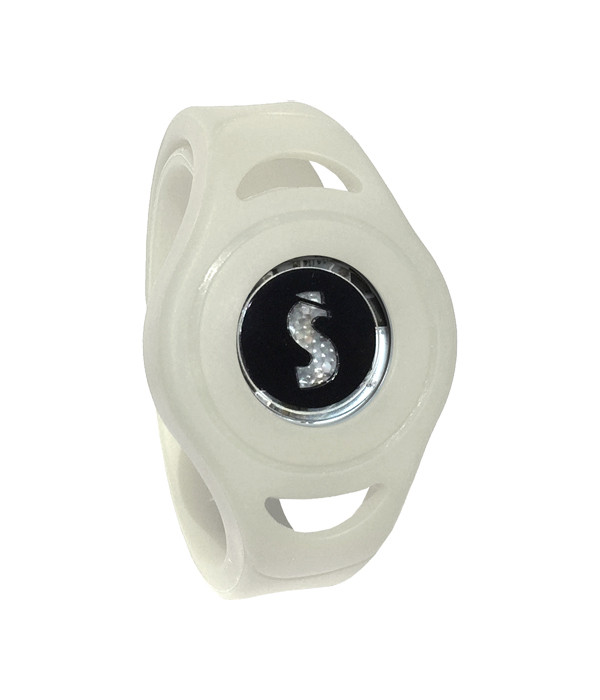
\includegraphics[scale=0.35]{figures/aProblemanalyse/sqord.JPG}
	\caption{På figuren ses The Sqord Booster sat i et armbånd. \citep{Sqord2016}}
	\label{fig:sqord}
\end{figure}
%Hjemmesiden hvor børnene kan følge med i deres avatar, fungerer som et forum, hvor de har mulighed for at give hinanden highfives for gode præstationer, chatte indbyrdes, eller lave talebobler, hvor alle kan se hvad de skriver. \citep{Sqord_family2015} \newline
The Sqord Booster tilgodeser alle præstationer, da alle får en medalje ved blot at have deltaget i en given aktivitet. Vinderen får imidlertid flere point end de andre deltagere. Spillet er lavet, så alle har mulighed for at vinde, da der i det enkelte spil, vurderes ud fra børnenes individuelle form, ved at se på tidligere præstationer. \citep{Sqord_family2015} \newline
The Sqord Booster har endvidere en indkøbspris på XXXX kr. 

\subsubsection{Vurdering af succeskriterier}
Aktivitetsmåleren registrerer både børnenes aktivitet ved gang og løb men kan ikke skelne mellem de to forskellige former for aktivitet, og der registreres ikke cykling. Der måles derudover ikke intensitet af det udførte arbejde, idet kun accelerometerets fart vurderes. \newline
Børnene bliver aktiveret socialt, da hjemmesiden er en blanding mellem et chatforum og en oversigt over præstationer. Derudover har børnene mulighed for at konkurrere med og mod hinanden. The Sqord Booster har derudover sørget for at fange både de børn der er i god form, og dem som ikke er, da alle har mulighed for at vinde baseret på tidligere præstationer. Aktivitetsmåleren er mulig at placere flere steder, hvormed børnene har mulighed for at vælge en placering, hvor det er til mindst gene.\fxnote{Derudover er det designet efter målgruppen, hvormed aktivitetsmåleren både kan modstå stød og tåle at komme i vand.}

The Sqord Booster opfylder to ud af seks succeskriterier, mens det delvist opfylder to succeskriterier.

\subsection{Nabi Compete}
Nabi Compete er en aktivitetsmåler, som appellerer til børn over seks år gennem deres madvaner og samvær med andre. Der er muligt for børnene at konkurrerer individuelt, men hovedformålet er at konkurrere mod eller med andre som et hold. Konkurrencerne kan bestå i at løbe en bestemt rute, som børnene selv kan designe og kan tegne ind. Desuden kan børnene vælge en fødevare i brugerfladen, og dermed vil brugerfladen fortælle barnet hvor meget det skal være fysisk aktiv for at have forbrændt kalorierne svarende til fødevaren. Der kan derfor være et konkurrende element i, at skulle forbrænde flest kalorier eller løbe længst.
%Det er muligt at opnå mål sammen med andre, eller dyste i hvem der når forskellige mål først. 
\fxnote{Derudover lærer børnene om kalorier og distance ved at bruge appen, hvor det er muligt at følge med i progressionen.}
Gennem konkurrencerne optjenes der point, som kan bruges til at købe et virtuelt dyr, som ved hjælp af point kan vokse. 
Aktiviteten måles gennem et tre-akse accelerometer, som sidder i et armbånd, hvilket kan ses på \figref{fig:nabi}. Dataet synkroniseres til en app gennem bluetooth, hvor der kan gemmes data i op til 90 dage, så barnet og forældrene dermed har mulighed for at følge med i barnets progression. \citep{Fuhu_tech2015,Fuhu2015} 
Nabi Compete har endvidere en indkøbspris på XXXX kr. 
\begin{figure}[H]
	\centering
	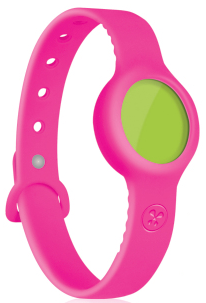
\includegraphics[scale=0.9]{figures/aProblemanalyse/nabi.png}
	\caption{På figuren ses Nabi Compete. \citep{Perez2015}}
	\label{fig:nabi}
\end{figure}

\subsubsection{Vurdering af succeskriterier}
Aktivitetsmåleren registrer både gang og løb, men det er ikke muligt at skelne mellem de to former for aktivitet, der registreres heriblandt ikke cykling eller intensitet med aktivitetsmåleren. 
Børnene aktiveres socialt, da appen er designet med mulighed for at konkurrere mod hinanden eller arbejde sammen i hold. Derudover har børnene mulighed for, 
%at have et kæledyr på appen, hvorved de, 
udover at konkurrere mod andre, kan se hvor mange kalorier de har forbrændt. Aktivitetsmåleren monteres uden gene, da den er placeret i en justerbar rem, som let kan monteres om barnets håndled.\fxnote{Derudover er den designet således at den kan tåle sved og regn, hvilket gør at børnene kan bruge det i al slags vejr.}

Nabi Compete opfylder to ud af seks succeskriterier, mens det delvist opfylder to succeskriterier.

\subsection{Ibitz}
Ibitz er en aktivitetsmåler, som apellerer til børn over fem år gennem udfordringer i samarbejde med forældrene. Ibitz har generelle udfordringer, men der lægges særligt op til at forældrene sætter nogle mål for børnene gennem deres dag og derved bestemmer udfordringerne. Forældrene har dermed mulighed for at lave en række opgaver til deres børn, som de vurderer er passende i forhold til barnets aktivitetsniveau. Barnet kan derfor vælge mellem disse tilpassede opgaver. \newline
Disse udfordringer kan indebære hvor meget tid børnene skal bruge på aktivitet og hvor land tid de må bruge på elektroniske spil. Ved at gennemføre udfordringerne forældrene eller Ibitz har sat, kan børnene tjene point, som kan bruges på to forskellige spil. \newline
%Dette kan være for hvornår der er legetid, hvornår de må sidde foran skærmen eller hvornår de skal lave aktiviteter med forældrene. 
Aktivitetsmåleren består af et pedometer, som måler skridt, der trådløst synkroniseres med en app via bluetooth. Aktivitetsmåleren monteres ved en klemme, som det fremgår af~\figref{fig:ibitz}. Appen gemmer aktiviteterne i 30 dage, hvorved barnet og forældrene har mulighed for at følge med i progressionen. \citep{Ibitz_features2016}
Ibitz har endvidere en indkøbspris på XXXX kr. 
\begin{figure}[H]
	\centering
	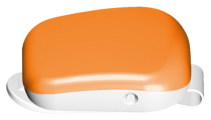
\includegraphics[scale=0.9]{figures/aProblemanalyse/ibitz.png}
	\caption{På figuren ses Ibitz klemmen.\citep{Ibitz_features2016}}
	\label{fig:ibitz}
\end{figure}

\subsubsection{Vurdering af succeskriterier}
Aktivitetsmåleren registrer både gang og løb, dog er det ikke muligt at skelne mellem de to former for aktivitet, samt at registrere puls og cykling. Børnene bliver delvist aktiveret socialt, hvor det primært er sammen med familien. Derudover aktiveres børnene ved at tjene point til forskellige spil, som oftest spilles sammen med andre børn. Aktivitetsmåleren monteres uden gene, da børnene selv kan vælge mellem at montere den på buksen eller skoen.\fxnote{Derudover kan den tåle vand, hvorved børn også kan bruge den i regnvejr}  

Ibitz opfylder to ud af seks succeskriterier, mens det delvist opfylder to succeskriterier.

\subsection{Samlet vurdering af de udvalgte aktivitetsmålere}
Ovenstående analyse og vurdering af de udvalgte aktivitetsmålere viser, at ingen af aktivitetsmålere opfylder alle de opstillede succeskriterier. \newline
Fælles for aktivitetsmålerne er, at de alle kan registrere løb og gang, men de kan dog ikke automatisk adskille disse aktivitetsformer. Yderligere var inden af aktivitetsmålerne i stand til at registrere cykling. \newline
Det er vurderet, at alle aktivitetsmålerne har en motiverende elementer således disse henvender sig til både fysisk aktivive og inaktive børn. \newline
Desuden kan alle aktivitetsmålerne monteres og placeres på komfortabel vis, således børnene ikke oplever gener ved at benytte dem. \newline
Indkøbsprisen for den enkelte aktivitetsmåler fremgår af nedenstående tabel. Denne pris vil kunne benyttes til at vurdere og sammenligne effektiviteten og prisen for de udvalgte aktivitetsmålere.  

%Ud fra vurderingen ses det, at de aktivitetsmålere, der i dag benyttes til børn i projektets aldersgruppe, ikke lever op til samtlige af de succeskriterier, som er stillet. De kan alle registrere løb og gang men har ikke mulighed for at skelne mellem de to aktivitetsformer. Ingen af aktivitetsmålerne registrerer cykling eller intensitet. Alle aktivitetsmålerne appellerer til både inaktive og aktive børn. Alle aktivitetsmålere er beregnet til at have rundt om armen, hvor den spændes på med en justerbar rem. Derudover er alle aktivitetsmålere designet efter, at børnene både skal kunne bruge dem i såvel regnvejr som solskin.

\begin{table}[H]
	\centering
	\resizebox{\textwidth}{!}{%
		\begin{tabular}{l c c c c}
			\rowcolor[HTML]{C0C0C0} 
			\multicolumn{1}{c}{\cellcolor[HTML]{C0C0C0}Krav} & \multicolumn{1}{c}{\cellcolor[HTML]{C0C0C0}Unicef Kid Power Band} & \multicolumn{1}{c}{\cellcolor[HTML]{C0C0C0}Sqord Booster}    &    \multicolumn{1}{c}{\cellcolor[HTML]{C0C0C0}Nabi Compete}     &   \multicolumn{1}{c}{\cellcolor[HTML]{C0C0C0}Ibitz} \\
			Registrere gang                                 & (x)                                        & (x)                                & (x)                               & (x)                        \\ \hline
			Registrere løb                                  & (x)                                        & (x)                                & (x)                               & (x)                        \\ \hline
			Registrere cykling                              &                                            &                                    &                                   &                            \\ \hline
			Registrere intensitet gennem puls               &                                            &                                    &                                   &                            \\ \hline
			Motivere inaktive såvel som aktive børn         & x                                          & x                                  & x                                 & x                          \\ \hline
			Monteres uden gene                              & x                                          & x                                  & x                                 & x                          \\ \hline
			Pris                                 & XXX kr.                                        & XXX kr.                               & XXX kr.                               & XXX kr.                      \\ \hline
		\end{tabular}
	}
	\caption{Tabellen viser en oversigt over de fire aktivitetsmålere, samt hvorvidt de lever op til succeskriterierne. (x) betyder, at de delvist lever op til succeskriterierne. x betyder, at de lever op til succeskriterierne}
	\label{tab:sammenhold_tracker}
\end{table}
For at optimere de aktivitetsmålere, der benyttes i dag, skal de kunne skelne mellem løb, gang og cykling, så barnet ikke kun kan måle, hvor mange skridt vedkommende har gået, eller hvor langt de er nået, men også kan måle hvilken aktivitet, som er udført. Derudover skal intensiteten af øvelsen kunne registreres ved hjælp af puls, da det har en afgørende betydning for det fysiologiske udbytte af den givne aktivitet, hvilket kan ses på \tabref{tab:PA_Procentpuls} i \secref{subsub:ak_int}.\newline
Aktivitetsmåleren skal, som de der findes i dag, aktivere børnene socialt sammen med jævnaldrende børn. Derudover skal aktiviteterne foregå igennem leg eller spil, som både skal være baseret på konkurrence mod andre eller sammenspil i hold. 